\section{An isolated sixth-order radial degeneracy and two radial extrema}
\label{rd:sec:main}

The existing fractional-turning analysis proves that the quadratic radial
coefficient has a unique zero in the outer order, and exhibits both signs
of the quartic coefficient along that threshold. Its final numerical
diagnostic suggests a simultaneous zero of those two coefficients near
$(a,b)=(1.00143,0.99749)$. We now certify that point, prove that it is
locally isolated, determine its sixth-order coefficient, and derive its
local radial geometry. In particular, some nearby fractional-order curves
have a strict local minimum followed by a strict local maximum. This is
a stronger failure of radial monotonicity than the previously proved
single-extremum branches.

The uniqueness asserted below is local to a stated rational rectangle.
No assertion about the total number of quartic transition points on the
full interval $0<b<1$ is needed or implied.

\subsection{A convergent all-orders equation for the radial coefficients}

For $a,b>0$, write
\[
 p_n=p_n(a,b)=\frac{H_{n-1}^{(b)}}{n^a},\qquad
 F_{a,b}(z)=\sum_{n\ge2}p_nz^n.
\]
Let $\theta_{a,b}(\rho)$ denote the unique zero of
$\Im F_{a,b}(\rho e^{i\theta})$ in the upper open semicircle, as
established by the manuscript's angular-zero theorem, and set
\[
 \eta_{a,b}(\rho)=\frac{\cos\theta_{a,b}(\rho)}{\rho},
 \qquad t=\rho^2.
\]
Only the local branch at $\rho=0$ is needed for the constructions below.
It can also be obtained directly by the implicit-function argument in
the following lemma.

\begin{lemma}[Binomial equation for every radial Taylor coefficient]
\label{rd:lem:allorders}
Define, for $j\ge0$,
\begin{equation}\label{rd:eq:Bj}
 B_j(v)=\sum_{k=0}^{j+1}(-1)^{j+1-k}\binom{j+1}{k}
                   (2v)^k p_{2j+3-k}.
\end{equation}
Near $t=0$, the radial zero is the analytic solution of
\begin{equation}\label{rd:eq:E}
 E(a,b,t,v):=\sum_{j\ge0}t^jB_j(v)=0,
 \qquad v(0)=\mu:=\frac{p_3}{2p_2}.
\end{equation}
The solution is jointly real analytic in $(a,b,t)$ near every point
with $a,b>0$ and $t=0$. Consequently
\begin{equation}\label{rd:eq:expansion}
 \eta_{a,b}(\rho)=\mu+K\rho^2+Q\rho^4+R\rho^6+O(\rho^8),
\end{equation}
where
\begin{align}
 K&=-\frac{B_1(\mu)}{2p_2},\label{rd:eq:K}\\
 Q&=-\frac{B_1'(\mu)K+B_2(\mu)}{2p_2},\label{rd:eq:Q}\\
 R&=-\frac{B_1'(\mu)Q+4p_3K^2+B_2'(\mu)K+B_3(\mu)}{2p_2}.
 \label{rd:eq:R}
\end{align}
In particular, at a simultaneous zero of $K$ and $Q$,
\begin{equation}\label{rd:eq:R0}
 R=-\frac{16p_5\mu^4-32p_6\mu^3+24p_7\mu^2-8p_8\mu+p_9}
          {2p_2}.
\end{equation}
\end{lemma}

\begin{proof}
Use $\sin(n\theta)=\sin\theta\,U_{n-1}(\cos\theta)$ and
the standard finite Chebyshev expansion~\cite{rd:DLMFChebyshev}
\[
 U_{n-1}(c)=\sum_{\ell=0}^{\lfloor(n-1)/2\rfloor}
   (-1)^\ell\binom{n-1-\ell}{\ell}(2c)^{n-1-2\ell}.
\]
Put $\cos\theta=\rho v$ and divide the imaginary-part equation by
$\rho^3\sin\theta$. A monomial indexed by $(n,\ell)$ has radial
power $\rho^{2(n-2-\ell)}$. For fixed $j=n-2-\ell$, write
$k=2j+3-n$. Then $0\le k\le j+1$, and the resulting coefficient
is exactly \eqref{rd:eq:Bj}.

The rearrangement gives a convergent analytic series, not only a formal
one. For real positive $a,b$, one may use $0<p_n\le n$. On a compact
complex neighborhood of a fixed positive parameter pair the same
coefficients have a uniform bound $|p_n|\le Cn^M$ for some finite $M$.
For $|v|\le V$ this bounds $|B_j(v)|$ by
$C(2j+3)^M(1+2V)^{j+1}$. Thus the series in \eqref{rd:eq:E}
converges normally when $|t|(1+2V)<1$.

Since $B_0(v)=2p_2v-p_3$, its $v$ derivative is $2p_2>0$.
The analytic implicit-function theorem applies and gives the stated
joint analyticity. Expanding $E$ to degree three in $t$ proves
\eqref{rd:eq:K}--\eqref{rd:eq:R}, because
\begin{align*}
 B_1(v)&=4p_3v^2-4p_4v+p_5,\\
 B_2(v)&=8p_4v^3-12p_5v^2+6p_6v-p_7,\\
 B_3(v)&=16p_5v^4-32p_6v^3+24p_7v^2-8p_8v+p_9,
\end{align*}
and $B_1''=8p_3$. Setting $K=Q=0$ gives \eqref{rd:eq:R0}.
\end{proof}

There is also a useful signed-moment interpretation. Whenever
$p_n=\int_0^1u^{n-1}\,d\nu(u)$ with $\nu([0,1])=0$,
the finite polynomial identity \eqref{rd:eq:Bj} becomes
\begin{equation}\label{rd:eq:momentBj}
 B_j(v)=\int_0^1\bigl[u(2v-u)\bigr]^{j+1}\,d\nu(u).
\end{equation}
Consequently a vanishing quadratic and quartic radial coefficient means
that the first three moments of the quadratic expression
$u(2\mu-u)$ vanish against this signed measure. The fourth such moment
determines the sixth radial coefficient by \eqref{rd:eq:R0}. The
finite-measure hypothesis holds at all parameter pairs used below.

\subsection{Exact isolation of the degeneracy}

All decimal endpoints in the next theorem denote terminating decimals,
hence exact rational numbers.

\begin{theorem}[Certified simultaneous zero and negative sixth coefficient]
\label{rd:thm:certificate}
There is exactly one pair $(a_\dagger,b_\dagger)$ in the open rectangle
\begin{align}
 1.00143018096149513812&<a<1.00143018096149513814,
 \label{rd:eq:abox}\\
 0.99749378987342042107&<b<0.99749378987342042108
 \label{rd:eq:bbox}
\end{align}
such that $K(a,b)=Q(a,b)=0$. At that point, and indeed throughout the
closed rectangle, the following rigorous bounds hold:
\begin{align}
 -3.368745\cdot10^{-11}&<R<-3.368744\cdot10^{-11},\label{rd:eq:Rbound}\\
 4.87028\cdot10^{-8}
  &<Q_b-Q_aK_b/K_a<4.87029\cdot10^{-8},\label{rd:eq:qprimebound}\\
 -8.31515\cdot10^{-10}
  &<K_aQ_b-K_bQ_a<-8.31513\cdot10^{-10}.
 \label{rd:eq:Jbound}
\end{align}
Moreover $K_a<0$, $K_b<0$, and $Q_a<0$ there. Thus the map
$(a,b)\mapsto(K,Q)$ is an analytic local coordinate system at
$(a_\dagger,b_\dagger)$, and the quartic coefficient crosses zero
strictly increasingly along the local branch $K=0$ as $b$ increases.
\end{theorem}

\begin{proof}
The accompanying verifier \texttt{certify\_radial\_degeneracy.py} uses
only Python's standard-library integer and rational arithmetic. Its
output, \texttt{radial\_degeneracy\_certificate.json}, records every
interval as exact rational endpoints, with a separate outward decimal
display. The finite computation and its analytic implications are as
follows.

Let $b_-$ and $b_+$ be the lower and upper endpoints in
\eqref{rd:eq:bbox}. The verifier encloses the corresponding zeros by
$L_-<a_*(b_-)<U_-$ and $L_+<a_*(b_+)<U_+$, where
\begin{align*}
 L_-&=1.00143018096149513813198112513591610363,\\
 U_-&=1.00143018096149513813198112513591610365,\\
 L_+&=1.00143018096149513812627198907246165442,\\
 U_+&=1.00143018096149513812627198907246165445.
\end{align*}
Specifically, $K$ is strictly positive at each lower $a$ endpoint and
strictly negative at each upper $a$ endpoint. The entire first thin
interval has $Q<0$, while the entire second has $Q>0$.

For transparency, the two quartic enclosures imply the simpler rational
inequalities
\[
 -2.244\cdot10^{-28}<Q(a_*(b_-),b_-)<-2.242\cdot10^{-28},
\]
\[
 2.626\cdot10^{-28}<Q(a_*(b_+),b_+)<2.629\cdot10^{-28}.
\]
Across the full closed rectangle, the verifier also proves
\begin{align*}
 -0.017073210967&<K_a<-0.017073210965,\\
 -0.009747328446&<K_b<-0.009747328443,\\
 -0.002284745315&<Q_a<-0.002284745313,
\end{align*}
as well as \eqref{rd:eq:Rbound}--\eqref{rd:eq:Jbound}.

Here are the elementary bounds underlying all transcendental
enclosures. For each integer $1\le n\le9$, put
$z=(n-1)/(n+1)$ and use the first $360$ terms of
\[
 \log n=2\sum_{j\ge0}\frac{z^{2j+1}}{2j+1}.
\]
The positive omitted tail is at most
$2z^{721}/(721(1-z^2))$. For every nonnegative rational argument
$x$ used in the computation, $x<3$. The Taylor polynomial for $e^x$
through degree $100$ has positive remainder at most
\[
 \frac{x^{101}}{101!}\frac{1}{1-x/102}.
\]
Exponentials at interval endpoints, followed by reciprocation, enclose
all powers $n^{-a}$ and $n^{-b}$. Each arithmetic operation is rounded
outward to integer multiples of $2^{-192}$. First derivatives are
enclosed by the ordinary product and quotient rules, starting from
\[
 \partial_a p_n=-(\log n)p_n,\qquad
 \partial_b p_n=-n^{-a}\sum_{m<n}(\log m)m^{-b}.
\]
Substitution in the finite formulas of Lemma~\ref{rd:lem:allorders}
therefore proves all recorded signs by finitely many rational
inequalities. No floating-point sign decision enters the certificate.

It remains to explain why these signs prove isolation. Since $K_a<0$
and $K_b<0$ throughout the rectangle, the endpoint brackets imply that
$K$ is positive on its lower $a$ edge and negative on its upper $a$
edge. For every $b\in[b_-,b_+]$ there is consequently a unique zero
$a_*(b)$ between those edges. The implicit-function theorem makes this
branch analytic and gives
\[
 a_*'(b)=-K_b/K_a.
\]
The quartic coefficient on it has derivative
$Q_b-Q_aK_b/K_a>0$ by \eqref{rd:eq:qprimebound}. Its opposite
endpoint signs give exactly one zero in $(b_-,b_+)$, and hence exactly
one simultaneous zero in the rectangle. Finally
\eqref{rd:eq:Jbound} gives the local inverse coordinate map, while
\eqref{rd:eq:Rbound} gives the negative sixth coefficient.
\end{proof}

\begin{remark}[What the certificate settles]
The original decimal location is upgraded to a proved rational
enclosure with local uniqueness, transversal quartic crossing, and a
nonzero sixth coefficient. The proof does not establish uniqueness of
the transition among all $0<b<1$. Nor does a local coefficient sign
prove monotonicity at every radius. The next results derive exactly the
local consequences warranted by these certified data.
\end{remark}

\subsection{A quarter-power branch of strict maxima}

Set
\[
 R_\dagger=R(a_\dagger,b_\dagger),\qquad
 r=-R_\dagger>0,\qquad
 \mu_\dagger=\frac{p_3(a_\dagger,b_\dagger)}
                   {2p_2(a_\dagger,b_\dagger)}.
\]

\begin{theorem}[Sixth-order decrease and quarter-power maximum birth]
\label{rd:thm:quarter}
At the certified pair,
\[
 \eta_{a_\dagger,b_\dagger}(\rho)
   =\mu_\dagger-r\rho^6+O(\rho^8),
\]
so the normalized-radius curve strictly decreases for sufficiently
small positive $\rho$. There are $\delta_0,\rho_0>0$ such that for
every $0<\delta<\delta_0$ the curve
$\eta_{a_\dagger-\delta,b_\dagger}$ has exactly one critical point
in $(0,\rho_0)$, a strict local maximum. Its radius is
\begin{equation}\label{rd:eq:quarter}
 \rho_{\max}(\delta)
 =\left(\frac{K_a(a_\dagger,b_\dagger)}{3R_\dagger}\right)^{1/4}
       \delta^{1/4}+O(\delta^{3/4}).
\end{equation}
The positive prefactor has the certified rational bounds
\[
 114.006986<
 \left(\frac{K_a(a_\dagger,b_\dagger)}{3R_\dagger}\right)^{1/4}
 <114.006989.
\]
For $a>a_\dagger$ sufficiently close, at the same $b=b_\dagger$,
there are no critical points in $(0,\rho_0)$ and the curve strictly
decreases there.
\end{theorem}

\begin{proof}
Write $\Phi(a,b,t)=\eta_{a,b}(\sqrt t)$ for the analytic solution
of Lemma~\ref{rd:lem:allorders}, and let $U=\partial_t\Phi$.
At the certified pair,
\[
 U(a_\dagger,b_\dagger,t)=3R_\dagger t^2+O(t^3).
\]
Moreover $U_{tt}=6R_\dagger<0$ at $t=0$. Choose a small fixed
parameter and $t$ rectangle on which $U_{tt}<0$, and then a positive
upper endpoint $t_0$ on which $U<0$ for all the sufficiently nearby
parameters considered here.

For $a=a_\dagger-\delta$, the initial value is
$U(a,b_\dagger,0)=K(a,b_\dagger)>0$. Strict concavity and the
negative value at $t_0$ imply exactly one zero in $(0,t_0)$; at it
$U_t<0$. Thus $\partial_\rho\eta=2\rho U$ changes from positive
to negative, giving a strict maximum.

To find its scale, put $\delta=s^2$ and $t=sv$. Analyticity makes
\[
 \frac{U(a_\dagger-s^2,b_\dagger,sv)}{s^2}
   =-K_a(a_\dagger,b_\dagger)+3R_\dagger v^2+O(s)
\]
an analytic expression through $s=0$. Its positive zero at $s=0$ is
$v_0=(K_a/(3R_\dagger))^{1/2}$ and has nonzero $v$ derivative.
The implicit-function theorem therefore gives
$v(s)=v_0+O(s)$. Taking the positive square root of
$t=\sqrt\delta\,v(\sqrt\delta)$ proves \eqref{rd:eq:quarter}.
The displayed prefactor enclosure is checked by comparing the fourth
powers of its rational endpoints against the exact interval for
$K_a/(3R)$; no numerical fourth root is required.

For $a>a_\dagger$ sufficiently close, both $K<0$ and $Q<0$,
because $K_a<0$ and $Q_a<0$ at the certified pair. Hence $U(0)<0$
and $U_t(0)=2Q<0$. Strict concavity forces $U<0$ throughout the
positive $t$ interval. At the certified pair itself, the leading term
$3R_\dagger t^2$ gives the stated strict decrease.
\end{proof}

\subsection{A proved region containing two radial extrema}

\begin{theorem}[A minimum followed by a maximum]
\label{rd:thm:two}
Use the analytic local coordinates $k=K(a,b)$ and $q=Q(a,b)$ centered
at $(a_\dagger,b_\dagger)$. There is an analytic function $\chi(q)$
near zero with
\begin{equation}\label{rd:eq:fold}
 \chi(q)=\frac{q^2}{3R_\dagger}+O(q^3)
        =-\frac{q^2}{3r}+O(q^3)
\end{equation}
and a fixed $\rho_0>0$ such that, for sufficiently small $q>0$:
\begin{enumerate}
\item If $\chi(q)<k<0$, the normalized-radius curve has exactly two
      critical points in $(0,\rho_0)$. The first is a strict local
      minimum and the second is a strict local maximum.
\item If $k=\chi(q)$, these two critical points coalesce at a positive
      radius. The derivative vanishes to order two there, and the
      curve strictly decreases through this stationary point.
\item If $k<\chi(q)$ and $(k,q)$ remains sufficiently near zero,
      the curve strictly decreases throughout $(0,\rho_0)$.
\end{enumerate}
In particular there is an explicit analytic parameter path
$(a(\varepsilon),b(\varepsilon))$ defined for small $\varepsilon>0$ by
\begin{equation}\label{rd:eq:scaledpath}
 K(a(\varepsilon),b(\varepsilon))=-\frac94r\varepsilon^2,
 \qquad
 Q(a(\varepsilon),b(\varepsilon))=3r\varepsilon.
\end{equation}
Its two critical radii satisfy
\begin{align}
 \rho_{\min}(\varepsilon)
   &=\sqrt{\varepsilon/2}+O(\varepsilon^{3/2}),\label{rd:eq:minscale}\\
 \rho_{\max}(\varepsilon)
   &=\sqrt{3\varepsilon/2}+O(\varepsilon^{3/2}).\label{rd:eq:maxscale}
\end{align}
All these parameters remain fractional positive orders with $a>1$ and
$0<b<1$ after the neighborhood is made sufficiently small.
\end{theorem}

\begin{proof}
Let $(a,b)=P(k,q)$ be the analytic inverse coordinate map guaranteed
by Theorem~\ref{rd:thm:certificate}, and continue to write
$\Phi(k,q,t)=\eta_{P(k,q)}(\sqrt t)$. Its derivative has the exact
analytic form
\[
 U(k,q,t)=k+2qt+3R(P(k,q))t^2+O(t^3).
\]
At the origin $U_{tt}=6R_\dagger<0$. Work in a small fixed rectangle
where $U_{tt}<0$ and with a positive endpoint $t_0$ where $U<0$
for all sufficiently small $(k,q)$.

The equation $U_t(k,q,t)=0$ has a unique analytic solution
$t=t_m(k,q)$ near the origin, because its $t$ derivative there is
$6R_\dagger\ne0$. Since $U_t(k,0,0)=0$ identically, uniqueness
gives $t_m(k,0)=0$. Expanding at the origin yields
\[
 t_m(k,q)=-\frac{q}{3R_\dagger}
               +O\bigl((|k|+|q|)^2\bigr).
\]
Thus $t_m>0$ for small $q>0$; more precisely $t_m=qA(k,q)$ with
$A$ analytic and $A(0,0)=-1/(3R_\dagger)>0$.

Define the local maximum value of $U$ by
$H(k,q)=U(k,q,t_m(k,q))$. Its derivative in $k$ at the origin is
one. The implicit-function theorem gives an analytic curve
$k=\chi(q)$ on which $H=0$, with $H>0$ for $k>\chi(q)$ and
$H<0$ for $k<\chi(q)$ nearby. Expanding $H$ gives
\[
 H(k,q)=k-\frac{q^2}{3R_\dagger}
                   +O\bigl((|k|+|q|)^3\bigr),
\]
and therefore \eqref{rd:eq:fold}.

If $\chi(q)<k<0$, then $U(0)=k<0$, its unique interior maximum
is positive, and $U(t_0)<0$. Strict concavity gives exactly two
simple positive zeros, with signs $- , + , -$ in the three intervening
intervals. Since $\partial_\rho\eta=2\rho U$, they are respectively
a strict minimum and a strict maximum. At $k=\chi(q)$ the maximum
equals zero, so the sole zero is double and $U$ is negative on both
sides. For $k<\chi(q)$ even its maximum is negative. These prove
the three local classifications. At the double zero $t_m>0$,
$U=U_t=0$ and $U_{tt}<0$; changing to $\rho=\sqrt t$ preserves
the multiplicity two of the first derivative.

The inverse map $P$ makes \eqref{rd:eq:scaledpath} an analytic path.
Put $t=\varepsilon v$. Along it, division by $3r\varepsilon^2$
gives an analytic expression through $\varepsilon=0$:
\[
 \frac{U(-\tfrac94r\varepsilon^2,3r\varepsilon,\varepsilon v)}
      {3r\varepsilon^2}
   =-\frac34+2v-v^2+O(\varepsilon).
\]
The two zeros at $\varepsilon=0$ are $v=1/2$ and $v=3/2$,
both simple. The implicit-function theorem yields
$v_-(\varepsilon)=1/2+O(\varepsilon)$ and
$v_+(\varepsilon)=3/2+O(\varepsilon)$. Positive square roots give
\eqref{rd:eq:minscale}--\eqref{rd:eq:maxscale}; concavity proves there
are no additional critical points in the chosen local interval.
Finally $(a_\dagger,b_\dagger)$ is strictly inside $a>1$, $0<b<1$,
so continuity preserves these inequalities in a small neighborhood.
\end{proof}

\subsection{An explicit rational pair with exactly two small-radius extrema}

The analytic parameter path above proves the mechanism. The following
independent certificate supplies a concrete rational pair and fixed
radial intervals. It encloses the actual implicit zero of $E$, including
the omitted infinite tail.

\begin{theorem}[A concrete minimum and maximum]
\label{rd:thm:explicit}
For the exact rational orders
\begin{equation}\label{rd:eq:explicitpair}
 a=1.0014289951689850677,\qquad b=0.9974958668828783544,
\end{equation}
the normalized-radius curve has exactly two critical points in
$0<\rho<\sqrt{7/4000}$. They are a strict local minimum and a strict
local maximum, respectively, with certified brackets
\begin{equation}\label{rd:eq:explicitbrackets}
 \frac1{\sqrt{4000}}<\rho_{\min}<\frac1{\sqrt{1000}}
 <\rho_{\max}<\sqrt{\frac7{4000}}.
\end{equation}
The assertion does not classify critical points at larger radii.
\end{theorem}

\begin{proof}
Put $\Phi(t)=\eta_{a,b}(\sqrt t)$ and $U(t)=\Phi'(t)$.
The verifier \mbox{\texttt{certify\_two\_extrema.py}} gives the exact
rational enclosures
\[
\begin{array}{c|c}
 t & \text{certified interval for }U(t)\\ \hline
 1/4000 & (-3.158,-3.156)\,10^{-17}\\
 1/1000 & ( 2.537, 2.538)\,10^{-17}\\
 7/4000 & (-3.136,-3.135)\,10^{-17}.
\end{array}
\]
Throughout the entire interval $0\le t\le7/4000$, it also proves
\begin{equation}\label{rd:eq:concavitycertificate}
 -2.1\cdot10^{-10}<\Phi'''(t)<-1.9\cdot10^{-10}.
\end{equation}
Here are complete bounds for the infinite series and implicit
calculation underlying these signs.

Sum \eqref{rd:eq:E} through $j=17$, so the omitted tail begins at
$N=18$. On $|v|\le1$ and $0\le t\le t_0:=7/4000$, any mixed
derivative with $r+s\le3$ has omitted tail bounded in absolute value
by
\begin{equation}\label{rd:eq:partialtail}
 T_{r,s}=15\left(\frac43\right)^s t_0^{-r}
       \frac{(3t_0)^N N^{r+s+1}(r+s+1)!}
            {(1-3t_0)^{r+s+2}}.
\end{equation}
To prove this, differentiate \eqref{rd:eq:Bj}, use $p_n\le n$ and
the binomial theorem, and write $(j)_r$ for the falling factorial.
For $j\ge N$ the resulting summand is at most
\[
 (j)_r(2j+3)2^s(j+1)_s3^{j+1-s}t_0^{j-r}
 \le15(4/3)^s j^{r+s+1}3^jt_0^{j-r}.
\]
For $q=3t_0$, $d=r+s+1$, and $j=N+\ell$, use
$j^d\le N^d(\ell+1)^d$ and
$(\ell+1)^d\le d!\binom{\ell+d}{d}$. Summing the binomial
generating function proves \eqref{rd:eq:partialtail}. The same
formula with each sample's smaller positive $t$ gives its sharper
pointwise bounds.

Every finite coefficient is enclosed using outward $192$-bit rational
interval arithmetic. The logarithms up to $\log37$ are evaluated by
binary range reduction: write $n=2^k y$, $1\le y<2$, and use
$\log n=k\log2+2\operatorname{arctanh}((y-1)/(y+1))$.
The last argument is less than $1/3$. One hundred terms of its positive
series, with the geometric tail used above, suffice. Exponentials use
one hundred Taylor terms and the same first-omitted-term geometric
bound; all arguments are less than five. Thus the powers and every
mixed derivative of the finite sum are rigorously enclosed.

The actual implicit root is trapped uniformly in the strip
\[
 0\le t\le7/4000,\qquad
 0.499999752369655\le v\le0.499999752369657.
\]
Including \eqref{rd:eq:partialtail}, the verifier proves $E<0$ on
the lower $v$ edge, $E>0$ on the upper edge, and $E_v>0$ throughout
the strip. Hence each $t$ has a unique root in this strip, depending
analytically on $t$; the angular-zero theorem identifies it with
$\Phi(t)$. At each sample point, a further rational $v$ bracket of
width $10^{-34}$ encloses the root. These finer brackets, edge signs,
and all derivative intervals are recorded in
\texttt{two\_extrema\_certificate.json}.

Implicit differentiation gives
\begin{align*}
 U&=-E_t/E_v,\\
 V:=\Phi''&=-\frac{E_{tt}+2E_{tv}U+E_{vv}U^2}{E_v},\\
 \Phi'''&=-\frac{E_{ttt}+3E_{ttv}U+3E_{tvv}U^2+E_{vvv}U^3
                       +3E_{tv}V+3E_{vv}UV}{E_v}.
\end{align*}
Substituting the exact mixed-derivative enclosures proves both the
three displayed signs and \eqref{rd:eq:concavitycertificate}.

Thus $U$ is strictly concave. Its signs $-,+,-$ force one zero in
each of $(1/4000,1/1000)$ and $(1/1000,7/4000)$. Strict concavity
permits no third zero and makes both zeros simple: the slope at the
first is positive, while the slope at the second is negative. Since
$\partial_\rho\eta=2\rho U$, they are exactly the asserted strict
minimum and maximum. Taking square roots of the $t$ brackets gives
\eqref{rd:eq:explicitbrackets}.
\end{proof}

\subsection{Scope and further questions}

These theorems answer the existing question about the higher radial
behavior at at least one quartic transition. They establish a certified
local configuration, analytic parameter families, and one explicit
rational pair with exactly two extrema on a fixed interval. The general
bifurcation theorems do not give uniform lower bounds on their
neighborhood sizes $\delta_0$, $\rho_0$, or the allowed
$\varepsilon$. The explicit example shows how convergent remainder
bounds can make an individual instance fully quantitative.

The next concrete research questions are:
\begin{enumerate}
\item Is the certified $b_\dagger$ the only zero of
      $Q(a_*(b),b)$ in $0<b<1$? The local uniqueness proof leaves
      the rest of that interval unclassified.
\item How many radial critical points can occur on the entire interval
      $0<\rho\le1$? The two-extremum theorem supplies a lower bound
      of two for the maximal possible count in the fractional family.
\item Can the integer-order all-radius monotonicity conjecture be
      proved from the positive double kernel or the one-change signed
      density? None of the present counterexamples has integer outer
      order.
\item Can the explicit two-extremum certificate be extended to a
      substantial open rational parameter rectangle, and can its
      critical radii be enclosed much more sharply? This would make
      the local bifurcation region quantitatively visible.
\item What is the analytic structure of the coefficient sequence near
      $(a,b)=(1,1)$, where $\eta\equiv1/2$ and every nonconstant
      radial coefficient vanishes? The nearby isolated degeneracy
      suggests studying that limit by a joint parameter expansion.
\end{enumerate}

\begin{figure}[tbp]
\centering
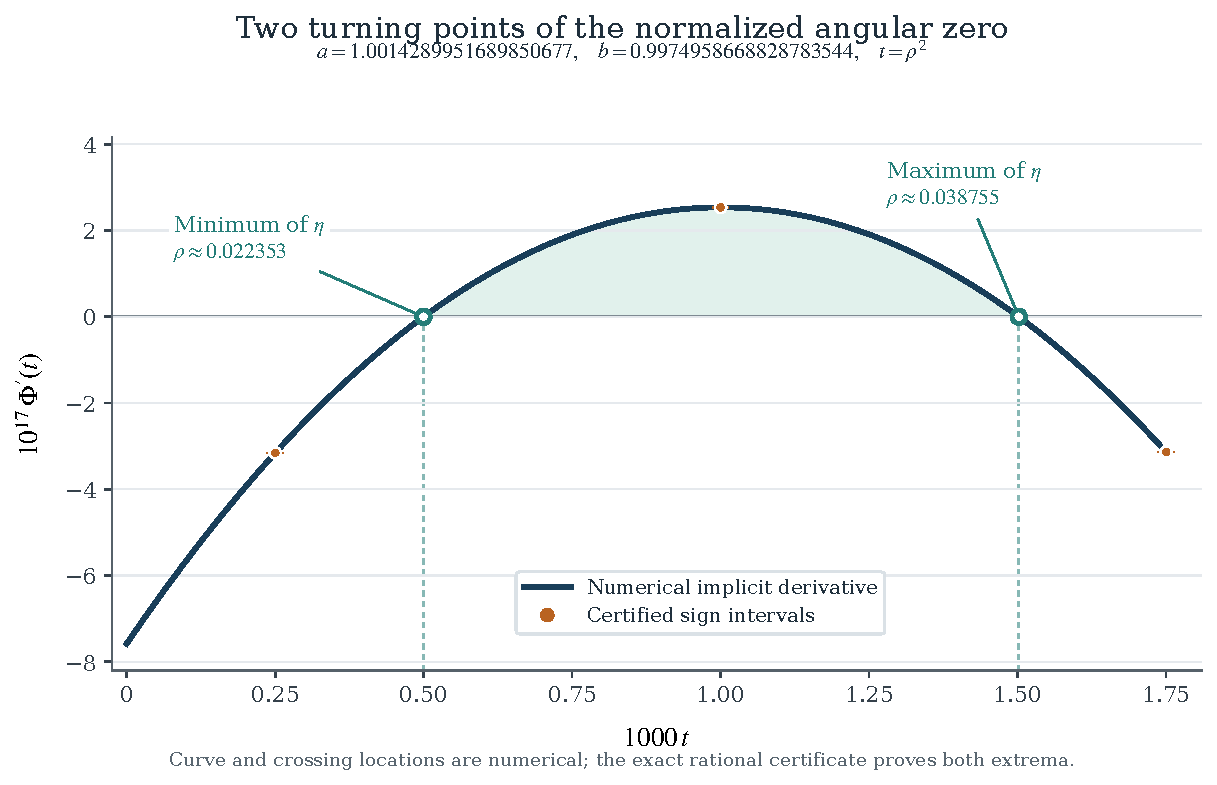
\includegraphics[width=\textwidth]{figures/radial_two_extrema.pdf}
\caption{The actual implicit derivative for the rational orders in
\eqref{rd:eq:explicitpair}. The blue curve and crossing locations
are numerical evaluations at 85 decimal digits; the orange markers
show the three exact rational sign enclosures. The independent
certificate proves $\Phi'''<0$ on the entire displayed interval,
so these signs establish exactly two simple critical points.
The much finer decimal crossing locations are diagnostic, not
additional certified radius brackets.}
\label{fig:radial-two}
\end{figure}
